\begin{frame}{Modello della rete}

\begin{columns}[c]

    \column{0.5\textwidth}
    Due popolazioni: \textit{hat} e \textit{check}\\
    Costi delle strade:
    \begin{equation*}
        \widehat{\tau}, \widecheck{\tau}: \mathbb{R}_+^N\times\mathbb{R}_+^N \to \mathbb{R}_+^N \cup \{+\infty\}
    \end{equation*}

    Costi dei percorsi:
    \begin{equation*}
        \begin{split}
        \widehat{T}(\theta)\coloneqq\widehat{\Gamma}^{\intercal}\widehat{\tau}(\widehat{\Gamma}\widehat{\zeta}\widehat{\theta},\widecheck{\Gamma}\widecheck{\zeta}\widecheck{\theta})\\
        \widecheck{T}(\theta)\coloneqq\widecheck{\Gamma}^{\intercal}\widecheck{\tau}(\widehat{\Gamma}\widehat{\zeta}\widehat{\theta},\widecheck{\Gamma}\widecheck{\zeta}\widecheck{\theta})
        \end{split}
    \end{equation*}

    \column{0.5\textwidth}
    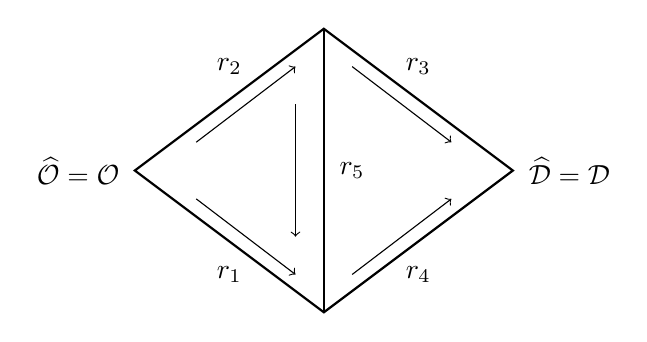
\begin{tikzpicture}[scale=1.2]

    \coordinate (L) at (0,0);
    \coordinate (T) at (2,1.5);
    \coordinate (R) at (4,0);
    \coordinate (B) at (2,-1.5);

    \draw[thick] (L) -- (T) -- (R) -- (B) -- cycle;
    \draw[thick] (T) -- (B);

    \draw[->] (0.65,0.3) -- (1.7,1.1);

    \draw[->] (0.65,-0.3) -- (1.7,-1.1);

    \draw[->] (2.3,1.1) -- (3.35,0.3);

    \draw[->] (2.3,-1.1) -- (3.35,-0.3);

    \draw[->] (1.7, 0.7) -- (1.7, -0.7);

    \node at (1,1.1) {$r_2$};
    \node at (1,-1.1) {$r_1$};
    \node at (3,1.1) {$r_3$};
    \node at (3,-1.1) {$r_4$};
    \node at (2.3, 0) {$r_5$};
    \node at (-0.6, 0) {$\widehat{\mathcal{O}} = \widecheck{\mathcal{O}}$};
    \node at (4.6, 0) {$\widehat{\mathcal{D}} = \widecheck{\mathcal{D}}$};
    \end{tikzpicture}

\end{columns}

\end{frame}